\section{Results and Discussion}
We were able to develop a library for simulating the kinematics of a system of rigid bodies. More specifically, we solved our project problem description, that is, we developed a library that could produce a kinematically admissible motion given a target motion and the definition of the rigid bodies in the system. To showcase our library, we developed the two more complex examples from the three originally proposed. These examples were a cube folding and a Miura origami pattern folding. The cube can fold well given five angular velocities related to the five joints that need to fold. The Miura pattern was difficult to fold into its iconic configuration due to the nature of the simulation. Due to how we implemented the library, most of the complexity of performing these simulations is in making the input file.

While the library is always able to simulate an admissible motion, it does not always simulate the motion you would expect from your defined target velocities. This makes the animation ``wiggly" in terms of the cube folding, and makes certain folding motions hard to achieve in terms of the Miura folding. Oftentimes, the target velocity that is specified is a scaled component of the usual basis of a space with a dimension equal to the number of degrees of freedom of your system. This target velocity will most likely not be in the null space of the constraint matrix, so it must be projected to it. When the size of the vectors in the null space becomes large (the degrees of freedom of the structure is large), it is difficult to determine where that vector will project. Sometimes it projects to an admissible velocity that would seem counterintuitive. If multiple target velocities are specified for the same time step, then achieving an admissible velocity that represents the motion desired becomes more feasible, but determining all those target velocities becomes cumbersome. 

The drawback of this library is mostly a feature of the method we chose to select an admissible velocity from all that is possible, which is to project on the null space. Many others are possible, such as using Lagrange multipliers to minimize a Newtonian equilibrium equation.

The rest of this section will be focused on presenting more specific results mirroring the work performed in the previous section, making sure to reflect on lessons learned, the usefulness of the work, and how it could be done better in the future.
\begin{figure}
    \centering
    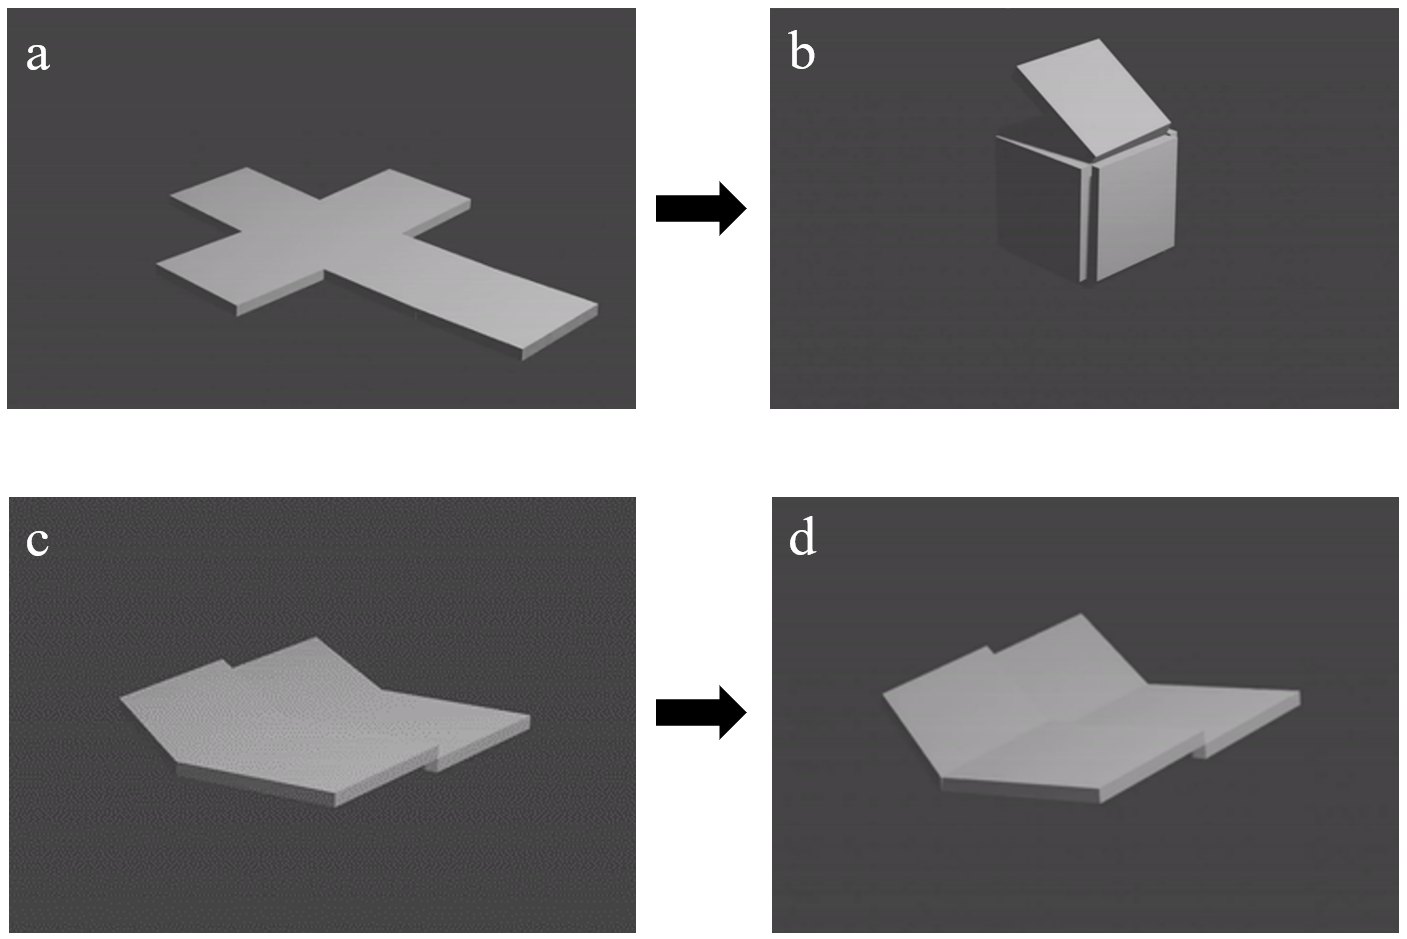
\includegraphics[width=0.9\linewidth]{Graphics/folding_examples.png}
    \caption{Example outputs from ori-kin library. (a) Shows unfolded cube example and (b) shows its folded state. (c) Shows unfolded Miura origami pattern example and (d) shows its partially folded state.}
    \label{fig:folding_examples}
\end{figure}

\begin{comment}
\begin{figure}
    \centering
    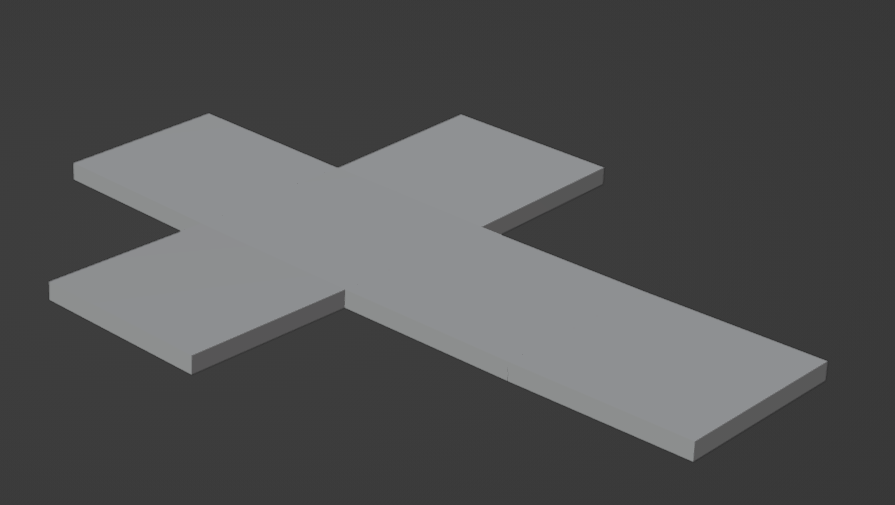
\includegraphics[width=0.5\linewidth]{Graphics/cube_unfold.png}
    \caption{Enter Caption}
    \label{fig:enter-label}
\end{figure}
\begin{figure}
    \centering
    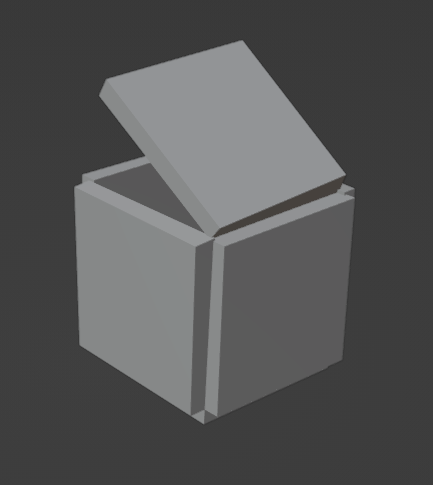
\includegraphics[width=0.5\linewidth]{Graphics/cube_fold.png}
    \caption{Enter Caption}
    \label{fig:enter-label}
\end{figure}
\begin{figure}
    \centering
    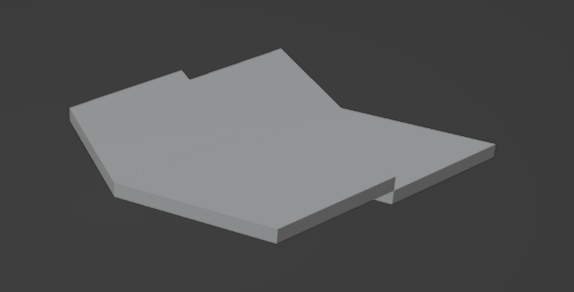
\includegraphics[width=0.5\linewidth]{Graphics/miura.png}
    \caption{Enter Caption}
    \label{fig:enter-label}
\end{figure}
\begin{figure}
    \centering
    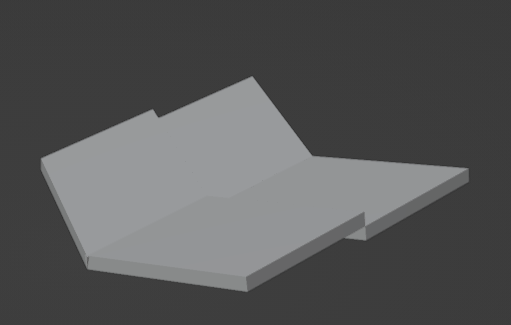
\includegraphics[width=0.5\linewidth]{Graphics/miura_fold.png}
    \caption{Enter Caption}
    \label{fig:enter-label}
\end{figure}
\end{comment}

\subsection{Waterfall Development Pattern}
The problem definition for our project was chosen as:``Develop a library to simulate the motion of constrained rigid bodies based on a given input motion."
We chose our high-level objectives to reflect the goals we had for our project in its proposal. The high-level requirements are the goals stated in the introduction.
% \begin{itemize}
%    \item The library shall be able to simulate the kinematics any convex rigid body that can be sufficiently described by its vertices.
%     \item The library shall make use of performant linear algebra libraries
%     \item The library shall make use of Object-Oriented Design
%     \item The library shall make use of design patterns
%     \item The library shall be extensible
%     \item The library shall use a CMake based build system
%     \item The library shall use C++ mainly and C if needed
% \end{itemize}

The functional requirements were developed to reflect the tasks defined in the proposal and any other requirements we realized after the fact. These functional requirements are as follows:

\begin{itemize}
    \item The library shall generate a complete mesh of a system of rigid bodies given an input file of each rigid body's relevant vertices.
    \item The library shall define a constraint matrix for a defined rigid body based only on the defined mesh and current position.
    \item The library shall compute a constrained set of velocities given a general velocity of interest and update the mesh positions based on a specified integration scheme.
    \item The library shall support calculations in double-precision arithmetic.
    \item The library shall provide a method for visualizing the constrained motion.
\end{itemize}

The library architecture, represented by our state and class diagrams, implemented a design we thought would be sufficient for our library. Ideally, we planned to only proceed through this process once since the library would be relatively simple. However, once we began the high and low-level design of our library, we quickly realized small modifications to the architecture would simplify the library's development. Because of this, we had to revert to the earlier architecture development steps to make these simplifications. In this sense, the final development pattern that was employed was closer to an iterative or agile one. This may have led to more efficiency overall because we did not need to spend excessive time in earlier development steps making sure we caught every detail, considering that most important details can't be seen until later steps. The final state and class diagrams are shown in Figures~\ref{fig:class}-\ref{fig:state}

\begin{figure} [H]
\centering
%\begin{minipage}{.5\textwidth}
  \centering
  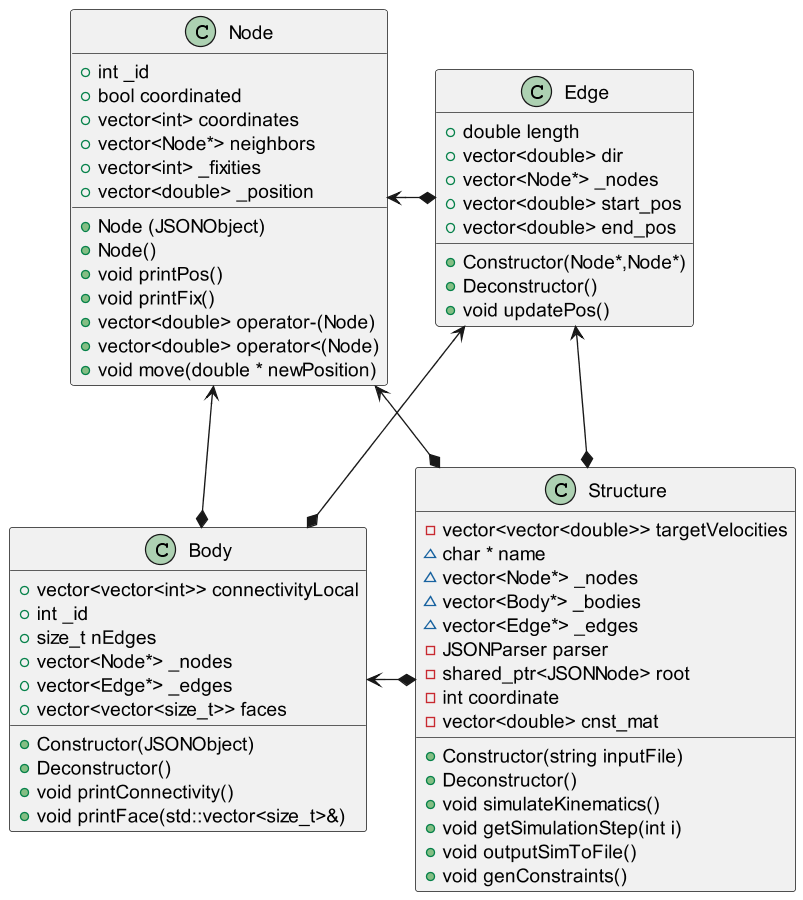
\includegraphics[width=0.7\linewidth]{Graphics/classNew.png}
  \captionof{figure}{UML class diagram of the most relevant classes in the ori-kin library}
  \label{fig:class}
  \end{figure}
%\end{minipage}%
%\begin{minipage}{.5\textwidth}
\begin{figure} [H]
  \centering
  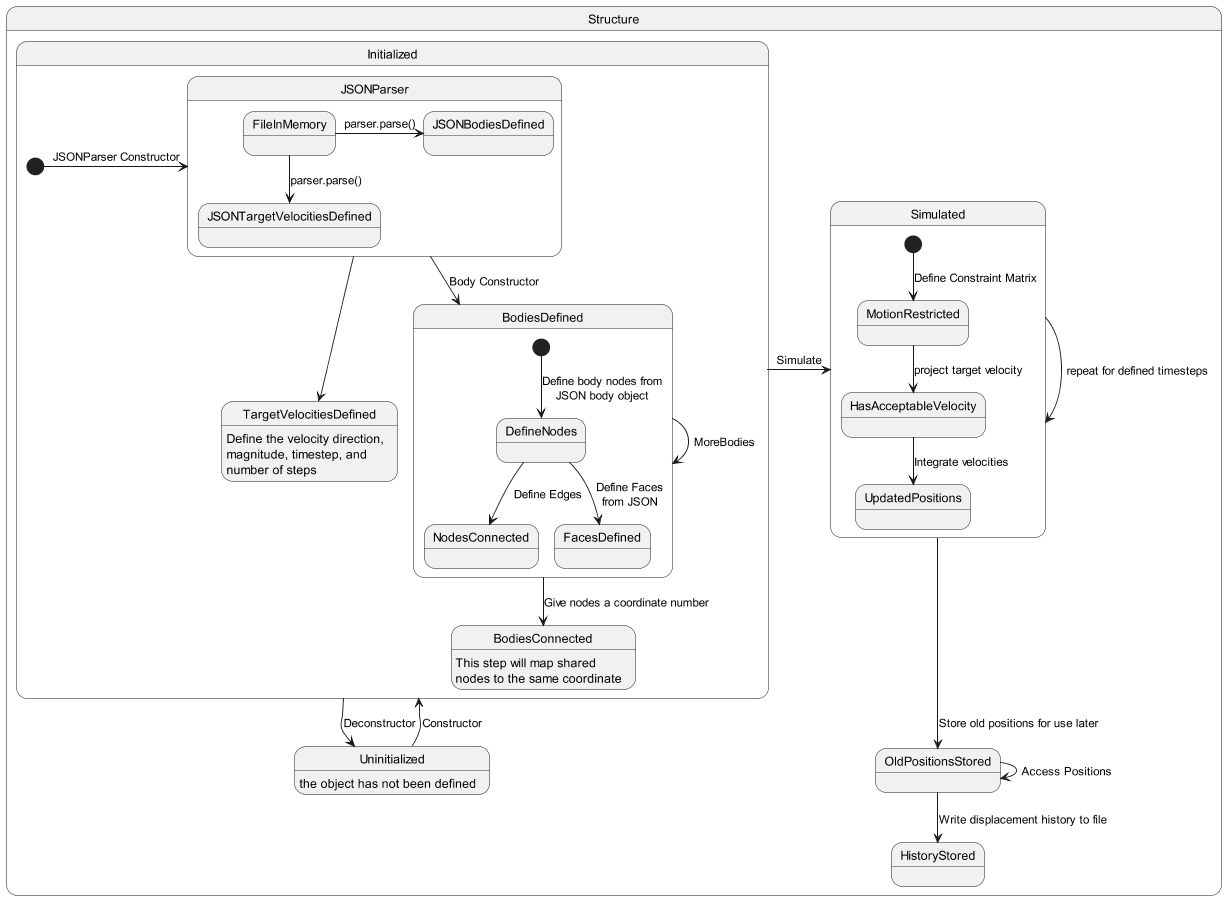
\includegraphics[width=0.7\linewidth]{Graphics/stateNew.png}
  \captionof{figure}{UML state diagram of a user's typical interaction with the library}
  \label{fig:state}
%\end{minipage}
\end{figure}
While the high-level requirements, functional requirements, and architecture were not critical to the library, taking the time to perform these non-essential earlier development tasks allowed for later essential tasks (high-level design, low-level design, etc.) to be completed more efficiently because we had a clear idea of how each component needed to interact with other components. Additionally, thinking through these earlier tasks likely reduced the amount of rework that would have been needed for this library.

\subsection{GitHub Repository}
Overall, our GitHub repository became more than a place to delegate work and combine our code. It became a place to work together and help solve each other's problems. The GitHub issues allowed for more than just task delegation. They also allowed us to completely describe and understand the task at hand before any code was written. Using GitHub projects, we could keep track of issues and manage their states more easily, allowing us to keep the project relatively on track. 

However, the management features of GitHub were mostly overkill, such as assigning labels, requiring reviews on pull requests, and putting issues in different bins. This is because we were a relatively small team with a relatively simple project, but using these features did give insight into how they can be useful on larger, ongoing projects that invite open-source collaboration and have issues submitted by people external to the core team. Besides using the issues to define the tasks well before we started working on them, most of the GitHub management features were done purely for housekeeping and provided no new information. The continuous integration features had a similar significance to the management features because we would have lengthy offline discussions about a branch before it was merged into the main one. In a larger, more distributed project, these features would have been critical.

The shared repository feature of GitHub was the most important for us. Using this feature, we could easily discuss problems we were having in our development by analyzing the changes made on someone's last commit. Then, we could propose our own changes based on a solution derived from our own expertise. For example, at one point, there was a bug in the branch responsible for developing the simulation method of the structure class. Jacob suspected there might have been an issue with the pseudo-inverse function, but was not as familiar with it as Noah, who implemented it. After committing his changes, Jacob asked Noah to review it to see if there is an issue. The issue was found and fixed quickly by Noah.
\subsection{Object-Oriented Design}
Using Object-Oriented Programming structures allowed us to combine data and functionality. This made developing the library more efficient because the data that was needed for an operation was easy to access. For example, during initialization, all the geometric and connectivity data for nodes, edges, and bodes are attached to their respective objects, and then their pointers are stored in a list as an attribute of the structure. This greatly simplifies the structure's generate constraint method. Instead of passing all the edges and nodes into the function by reference, they are automatically in the scope of the method and can be called directly. Furthermore, the nodes' and edges' attributes can be easily accessed too.
\begin{verbatim}
void Structure::genConstraints(){
...
full_cnst_mat[i][j] = _edges[i]->start_pos[0]-_edges[i]->end_pos[0];
...
}
\end{verbatim}

Special methods could also be implemented for each object to simplify common operations on the object's attributes. For example, the difference in node positions often needed to be computed, so instead of manually iterating through each position for every occurrence of this operation, we overloaded the subtraction operator on the node class so that node objects could be subtracted and a vector representing their difference could be returned
\begin{verbatim}
vector<double> Node::operator-(Node input){
    vector<double>res{0.0,0.0,0.0};
    for (int i=0;i<3;i++){
        res[i]=_position[i]-input._position[i];
    }
    return res;

}
\end{verbatim}

One of the biggest features of object-oriented programming is encapsulation, however, due to limited development time, we had to make most of the variables public for testing purposes. The alternative to this would be to make specific accessors for each variable we wanted to test. Not implementing this feature of object-oriented programming will make the software more susceptible to misuse by users and result in errors that are not obvious or caught by the program. 
\subsection{Compilation and External Libraries}
Using CMake made our library more portable, easier to recompile, and easier to integrate external libraries. 
We chose to use LAPACK and OpenBLAS external libraries \cite{anderson1999lapack} to perform the linear algebra operations since they are open source libraries with more mature algorithms than anything we could develop in the given time frame. The LAPACKE and cBLAS wrappers were used for this work. LAPACKE required input matrices to be passed as column-major or row-major arrays. We chose to pass them as column-major arrays which then set the format requirement for the rest of the library. Linear-algebra functions were then written in C++ that call the \texttt{cblas\_dgemm(...)} and \texttt{LAPACKE\_dgesdd(...)} routines. Each function took in column-major vectors rather than arrays to avoid memory leaks and converted them within the function. A pseudo inverse function did not exist in LAPACKE, so we wrote the function ourselves by calling \texttt{LAPACKE\_dgesdd(...)} for the decomposition and performed respective matrix multiplication with cBLAS. Figure \ref{fig:compilation} shows the flow of information in the CMake and Make process. The main workspace contained all the source and header files, which was added to the CMake sub-directories in the CMakeList. From the project workspace, we executed \texttt{cmake -S. -B./build} which then created the build directories which had the same file structure as the main project workspace. This build directory is system-dependent, and is ignored by Git when code is pushed to the repository. From the build file we then went into each source directory and executed the \texttt{make} command which then created the executables.
\begin{figure}[H]
\centering
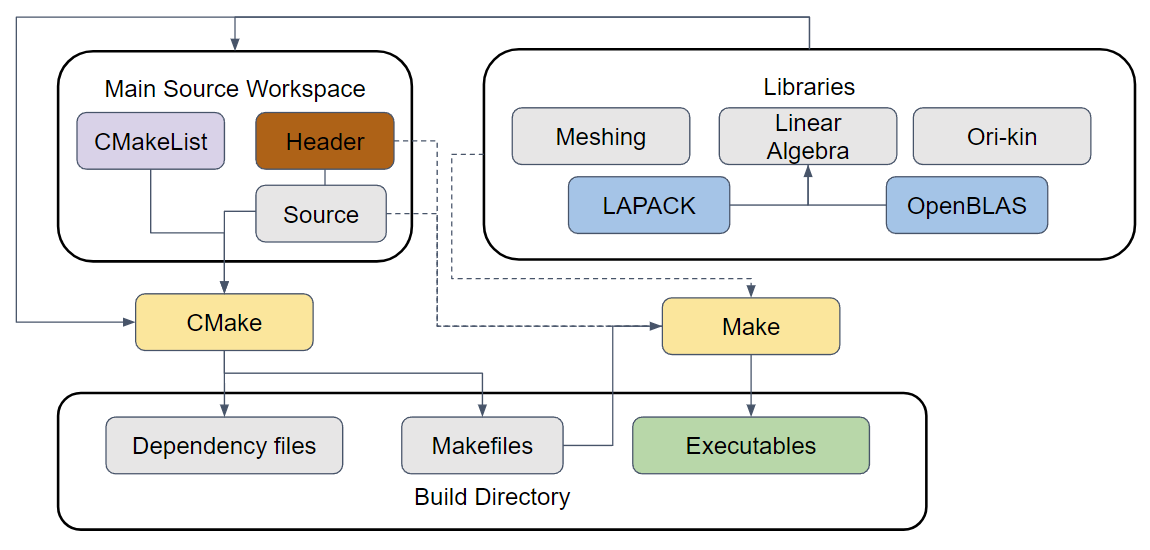
\includegraphics[width=0.8\textwidth]{Graphics/cmake.PNG}
\caption{CMake compiling flow chart for the ori-kin library}
\label{fig:compilation}
\end{figure}
\subsection{Visualization}
As seen in Figure \ref{fig:folding_examples}, we were successfully able to visualize our simulations using the Python scripting language and the Blender executable. This part of our library is important because it is the main medium of interpreting the simulation results. While the script is capable of producing animations, It is much less accessible than our library. The visualization script has static file paths to the output JSON file and output video file, it needs to have a Python version 3.10 library installed with the bpy module, and it must be called explicitly after a simulation to produce an animation. Ideally, these are all issues that could be resolved during the project configuration using CMake, but we did not reach this point in our project. For another user to make an animation with our library, they will need to understand the background processes well, which is bad programming philosophy and does not follow the key ideas of abstraction.
\subsection{Testing}
Testing is a critical step in software design and development. It enables us to find issues quickly and also helps benchmark the code so that when new functionalities are implemented, we can go back to the prior tests and ensure every component is working adequately. It is for this reason that testing cases are implemented with the library. This work details the unit and verification testing of the ori-kin library. We chose to put more emphasis on unit testing so that it would be easier to find small issues that novice programmers (like ourselves) make. 
\subsubsection{Unit Tests}
Unit tests were designed to catch small errors in the routines used throughout the library. These tests were designed to check if a function works in isolation, and therefore does not verify that it would work concurrently with other functions. The five main categories for the unit tests are the parser, meshing, constraint, simulation, and linear algebra tests.
The unit tests for the latter categories consisted of the following tests listed in Tables \ref{tab:meshing_ut}-\ref{tab:linalg_ut}. In the tables, each of their intended checks are described. These tests helped us out greatly, as we found several bugs/errors in all categories. For example, the linear algebra test found an error in linking the LAPACKE library that was not caught in the compilation, the constraints test resolved a bug where the fixities were being assigned but the constraint matrix was not properly sized so it was unable to incorporate the fixities, and so forth. Many unit tests require that geometry is generated from the meshing algorithm. The test mesh used was a simple unit cube. With this simple geometry, we are able to manually verify what the expected output of each function should be.
\subsubsection{Verification Tests}
The verification tests are done to check that the functions work together in a main program that uses multiple functions. This catches errors that unit tests are not able to catch, such as improper variable deallocation, memory leakage, and other hosts of problems. Several sets of verification were implemented in a verification test executable. These tests used a simple cube mesh. The overall projection step using the linear algebra, ODE, and accessor functions was tested by manually computing the expected matrices along each step of the multi-function process and comparing the results with assert statements. This was a major component of the \texttt{Structure.simulate()} function which runs the actual simulation and relies on many other classes and functions. Next, the deallocation features in the linear algebra were also tested, where multiple subsequent uses of the linear algebra functions were compared against a known solution. These tests helped find several memory leaks and deallocation issues. For example originally we passed standard arrays into the linear algebra functions, but when used sequentially, gave errors as some arrays had random values after it was used once in a function. This was resolved by converting storage to vectors and led to discoveries of bugs where we forgot to delete unused memory. Finally the last verification was to ensure the edge lengths remained roughly constant. A rigid treatment means that their change in length should be zero, but it is known that the first-order Euler solver introduces error when solving the ODE, so we expect an error that scales with the number of iterations, but plateaus and remains nearly constant once the kinematics are no longer in motion. Results for this error are shown in Figure \ref{fig:euler-error}, where the expected trend is shown. Finally, proof of all tests passing in GitHub checking is shown in Figure \ref{fig:test-pass}.

\begin{table}[H]
\centering
\caption{Meshing Unit Tests}
\label{tab:meshing_ut}
\def\arraystretch{1.05}
\makebox[\textwidth][c]{
\begin{tabular}{|c|c|}
\hline
\textbf{Test name}                   & \textbf{Purpose} \\ \hline
nodeOrder & ensures node ordering follows expected convention  \\ \hline
allHere   & ensures the right number of bodies and nodes are created  \\ \hline
nodeInit   & checks if nodes positions are correct and if fixites are created  \\ \hline
nodeSub   & checks that distance between nodes is correct  \\ \hline
nodeComp   & checks if node comparsion is valid both ways  \\ \hline
edgeInit   & ensures edge lengths are created correctly  \\ \hline
edgeUpdate   & checks if direction, length, and psoition are correctly updated   \\ \hline
bodyInit   & ensures that faces are correctly created \\ \hline
allCoordinated   &  tests each node to see if coordinated \\ \hline
jointDefined   & ensures node joints are the same value  \\ \hline
\end{tabular}
}
\end{table}

\begin{table}[H]
\centering
\caption{JSON Parser Unit Tests}
\label{tab:parse_ut}
\def\arraystretch{1.05}
\makebox[\textwidth][c]{
\begin{tabular}{|c|c|}
\hline
\textbf{Test name}                   & \textbf{Purpose} \\ \hline
stringParser & checks if strings are correctly read  \\ \hline
listParser & checks if correct string lengths are obtained \\ \hline
nestObjParse & checks if objects are correctly accessed in nest\\ \hline
nestNumPars & checks if object numbers are correctly accessed in nest\\ \hline
trueParse & ensures a true bool value is correctly parsed\\ \hline
falseParse & ensures a false bool value is correctly parsed\\ \hline
multiNestParse & checks if a double nested object is correctly accessed \\ \hline
printJson & checks it parsed output matches read-in file\\ \hline
\end{tabular}
}
\end{table}

\begin{table}[H]
\centering
\caption{Kinematic Simulation/Constraints Tests}
\label{tab:kinsim-con_ut}
\def\arraystretch{1}
\makebox[\textwidth][c]{
\begin{tabular}{|c|c|}
\hline
\textbf{Test name}                   & \textbf{Purpose} \\ \hline
checkCols & ensures that the correct number of rows is created in constraint matrix for test mesh  \\ \hline
checkRow   & checks if the one the the rows is correctly populated based on node coordinates  \\ \hline
projection & checks to see if math for projection onto null-space is correct  \\ \hline
velocityVectorInit & ensures velocity type and values and time stepsize are correctly initalized \\ \hline
normalizeTest & check if normalization is correct  \\ \hline
projectTest & checks to see if projection of two vectors is correct \\ \hline
updateAngle & checks if angle change gives correct velocity change  \\ \hline
strucutreVelAccess & checks functionality of velocity accessor  \\ \hline
\end{tabular}
}
\end{table}

\begin{table}[H]
\centering
\caption{Linear Algebra Unit Tests}
\label{tab:linalg_ut}
\def\arraystretch{1.05}
\makebox[\textwidth][c]{
\begin{tabular}{|c|c|}
\hline
\textbf{Test name}                   & \textbf{Purpose} \\ \hline
pseudoInv & check if pseudo inverse is correct for non-trivial tall-rectangular matrix  \\ \hline
pseudoInvNGrM   & check if pseudo inverse is correct for non-trivial long-rectangular matrix  \\ \hline
matMult  & checks if matrix-matrix multiplication of non-trivial non-square matrix is correct  \\ \hline
matVec   & checks if matrix-vector multiplication of non-trivial matrix is correct  \\ \hline
\end{tabular}
}
\end{table}

\begin{figure}
\centering
\begin{minipage}{.5\textwidth}
  \centering
  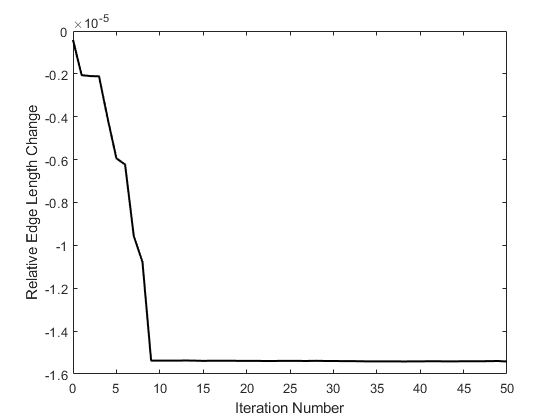
\includegraphics[width=1\linewidth]{Graphics/euler-error.png}
  \captionof{figure}{Change in edge length with respect to number of iterations for a step size of 0.01}
  \label{fig:euler-error}
\end{minipage}%
\begin{minipage}{.5\textwidth}
  \centering
  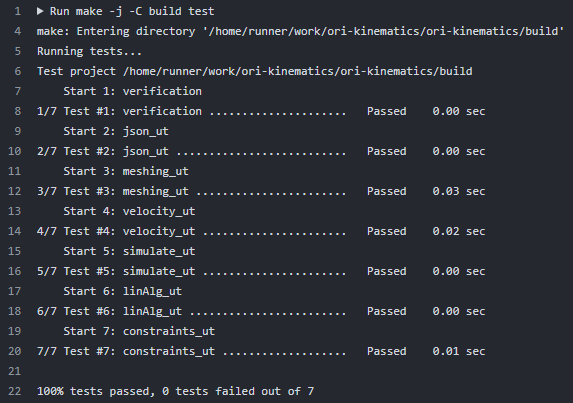
\includegraphics[width=1\linewidth]{Graphics/test-pass.PNG}
  \captionof{figure}{Output of passed tests in GitHub}
  \label{fig:test-pass}
\end{minipage}
\end{figure}